\documentclass[10pt]{beamer}

\usetheme[progressbar=frametitle]{metropolis}

\usepackage{booktabs}
\usepackage[scale=2]{ccicons}

\usepackage{pgfplots}
\usepgfplotslibrary{dateplot}

\usepackage{xspace}
\newcommand{\themename}{\textbf{\textsc{metropolis}}\xspace}

\title{The Alexander Polynomial}
\subtitle{And all that jazz}
\date{\today}
\author{Justin and Leigh}
\institute{Seattle University}
\titlegraphic{\hfill
\includegraphics[height=1.5cm]{SU_logo.png}}

\begin{document}

\maketitle

\begin{frame}{Table of contents}
  \setbeamertemplate{section in toc}[sections numbered]
  \tableofcontents[hideallsubsections]
\end{frame}

\section{Defining the Polynomial}

\begin{frame}[fragile]{Assembling The Matrix}
\begin{itemize}
  \item Start with an oriented knot diagram
  \item Label all the crossings 1, 2, ..., n
  \item Label all the regions 1, 2, ..., n, n+1, n+2
  \item Create an n x n+2 matrix where the rows correspond to crossings,
  the columns correspond to regions.
  \end{itemize} 
\end{frame}

\begin{frame}[fragile]{Assembling The Matrix}
  Each entry in the matrix will be determined by the labels defined in Figure 1.
  \begin{figure}
  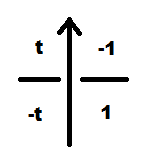
\includegraphics {crossing_labelings.png}
  \caption{Matrix Entries}
  \end{figure}
  At each row, all other regions that do not intersect with the specific crossing have a value of zero.
\end{frame}

\begin{frame}[fragile]{Assembling The Matrix}
\begin{itemize}
\item Delete two columns of the matrix corresponding to adjacent regions
\item The resultant n x n matrix is the Alexander Matrix
\item The determinant of the Alexander Matrix is the Alexander Polynomial
\item Depending on which columns are deleted, the determinant may differ by a factor of $ \pm t^k $
\item Conclude by dividing by the largest possible power of $t$ and factoring out a $-1$ if necessary to make the constant positive
\end{itemize}
\end{frame}

\section{Example}

\begin{frame}[fragile]{Trefoil Knot}
	\begin{figure}
    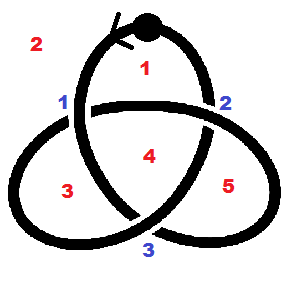
\includegraphics[scale=0.5]{Labeled_Trefoil_2}
    \caption{Labeled Trefoil}
    \end{figure}
\end{frame}

\begin{frame}{Corresponding Matrix and Determinant}
	\begin{figure}
    \centering
    \[
    M=
    \begin{bmatrix}
    -t & 1 & -1& t & 0\\
    -1 & 1 & 0 & t & -t\\
    0 & 1 & -t & t & -1
    \end{bmatrix}
    \]
    \end{figure}
    \pause
    \begin{figure}
    \centering
    \[
    Alexander Matrix=
    \begin{bmatrix}
    -t & 1 & -1\\
    -1 & 1 & 0\\
    0 & 1 & -t
    \end{bmatrix}
    \]
    \end{figure}
    \pause
   $$ \text{Det(Alexander Matrix)} = t^2 - t + 1 $$
\end{frame}

\section{Reidemeister Moves}

\begin{frame}[fragile]{Delta-Equivalent Matrices}
\begin{itemize}
\item Two matrices have the same determinant if they are delta-equivalent and one can be transformed into another by a sequence of the following moves:
\item Multiple a row or column by k.
\item Swapping two rows or columns.
\item Add one row or column to another.
\item Add or remove corner.
\item Multiply or divide a column by t.
\end{itemize}
\end{frame}



\begin{frame}[fragile]{Reidemeister 1 Move}
     \begin{figure}
     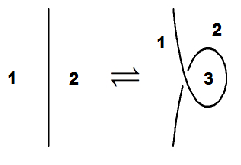
\includegraphics[scale=0.5]{R1.png}
      \caption{Reidemeister 1 move}
\end{figure}  
\begin{itemize}
\item Notice that the R1 move adds one new crossing and one new region
\item This corresponds to one new row and one new column in the matrix
\item Choose to delete regions 1 and 2 from the matrix 
\item The new Alexander matrix will have one row and column which only contains only $1, -1, t, or -t$ 
\item Thus the determinant will differ by a factor of $  -1 $
\end{itemize}
\end{frame}

\begin{frame}{Reidemeister 2 Move}
  \begin{figure}
  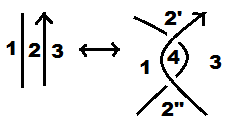
\includegraphics[scale=0.5]{R2_2.png}
  \caption{Reidemeister 2 move}
\end{figure}
\begin{itemize}
\item Notice that the R2 move adds 2 new crossings, 1 new region, and splits an existing region into two regions
\item Choose to delete region 1 and one of the split regions. We will choose to delete region 2'
\end{itemize}
\end{frame}

\begin{frame}{Reidemeister 2 Move}
  \begin{figure}
  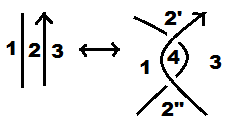
\includegraphics[scale=0.5]{R2_2.png}
  \caption{Reidemeister 2 move}
  \end{figure}
  \begin{itemize}
  \item For the given orientation, the entries in the new rows of the matrix are as follows:
  \[
  M=
  \bordermatrix{ & 2" & 3 & 4 \cr
  & 0 & -1 & 1 \cr
  & -t & 1 & -1 } \qquad
  \]
  \item The remaining entries in these rows are all zero
  \item Columns 2" and 3 have nonzero entries below these
  \end{itemize}
\end{frame}

\begin{frame}{Reidemeister 2 Move}
\begin{itemize}
\item We can add column 4 to column 3
  \[
  M=
  \bordermatrix{ & 2" & 3 & 4 \cr
  & 0 & 0 & 1 \cr
  & -t & 0 & -1 } \qquad
  \]
  \item Then we can add column 2` to column 4
  \[
  M=
  \bordermatrix{ & 2" & 3 & 4 \cr
  & 0 & 0 & 1 \cr
  & -t & 0 & 0 } \qquad
  \]
  \item Next divide row 2 by -t
  \[
  M=
  \bordermatrix{ & 2" & 3 & 4 \cr
  & 0 & 0 & 1 \cr
  & 1 & 0 & 0 } \qquad
  \]
  \end{itemize}
\end{frame}

\begin{frame}{Reidemeister 2 Move}
  \[
  M=
  \bordermatrix{ & 2" & 3 & 4 \cr
  & 0 & 0 & 1 \cr
  & 1 & 0 & 0 } \qquad
  \]
  \begin{itemize}
  \item When calculating the determinant, expand across the rows with only one nonzero entry
  \item The determinant will now be unchanged from an R2 move up to a factor of $ \pm t^k $
  \end{itemize}
\end{frame}

\begin{frame}{Reidemeister 3 Move}
\begin{figure}
  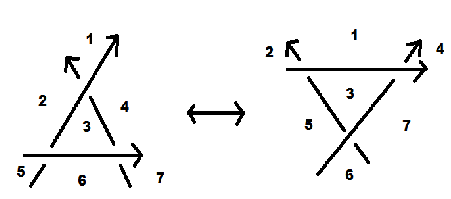
\includegraphics[scale=0.5]{R3.png}
  \caption{Reidemeister 3 move}
  \end{figure}
   \begin{itemize}
 \item The R3 move changes the matrix dramatically that we fail to identify.
\item Notice that two matrices are delta-equivalent if the corresponding matrices with all positive entries are delta-equivalent.


\end{itemize}
\end{frame}

\begin{frame}{Reidemeister 3 Move}

   \begin{itemize}
\item Due to checkerboard coloring and the way we index the regions around each crossing, we can multiple each odd column by -1 so that each row will have only positive or negative entries.
\item We can get a new matrix with non-negative entries by multiplying all negative rows by -1.

\end{itemize}
\end{frame}





\begin{frame} {Reidemeister 3 Move}
  \begin{itemize}
  \item For the given orientation, the entries in the relevant rows of the original matrix are as follows:
  \[
  M=
  \bordermatrix{ & 1 & 2 & 3 & 4 & 5 & 6 & 7 \cr
  & 0 & -t & t & 0 & 1 & -1 & 0  \cr
  & 0 & 0 & -t & t & 0 & 1 & -1  \cr
  & t & -t & 1 & -1 & 0 & 0 & 0
 } \qquad
  \]
  \item The remaining entries in these rows are all zero
  \item Only the remaining entries in column 3 are all zero.
  \end{itemize}
\end{frame}

\begin{frame} {Reidemeister 3 Move}
  \begin{itemize}
  \item For the given orientation, the entries in the relevant rows of the matrix after R3 move are as follows: 
  \[
  N=
  \bordermatrix{ & 1' & 2' & 3' & 4' & 5' & 6' & 7' \cr
  & -t & 0 & 1 & t & 0 & 0 & -1  \cr
  & t & -t & -1 & 0 & 1 & 0 & 0  \cr
  & 0 & 0 & t & 0 & -t & 1 & -1
 } \qquad
  \]
  \item Again, the remaining entries in these rows are all zero and Only the remaining entries in column 3' are all zero.
  \item Notice that all entries in other columns remain constant by R3 move.
  \end{itemize}
\end{frame}

\begin{frame} {Reidemeister 3 Move}
  \begin{itemize}
  \item Identify whether these two matrices with all positive entries are delta-equivalent.
  \[
  M'=
  \bordermatrix{ & 1 & 2 & 3 & 4 & 5 & 6 & 7 \cr
  & 0 & t & t & 0 & 1 & 1 & 0  \cr
  & 0 & 0 & t & t & 0 & 1 & 1  \cr
  & t & t & 1 & 1 & 0 & 0 & 0
 } \qquad
  \]
 \[
  N'=
  \bordermatrix{ & 1' & 2' & 3' & 4' & 5' & 6' & 7' \cr
  & t & 0 & 1 & t & 0 & 0 & 1  \cr
  & t & t & 1 & 0 & 1 & 0 & 0  \cr
  & 0 & 0 & t & 0 & t & 1 & 1
 } \qquad
  \]

  \end{itemize}
\end{frame}

\begin{frame} {Reidemeister 3 Move}
  \begin{itemize}
  \item
  \[
  M'=
  \bordermatrix{ & 1 & 2 & 3 & 4 & 5 & 6 & 7 \cr
  & 0 & t & t & 0 & 1 & 1 & 0  \cr
  & 0 & 0 & t & t & 0 & 1 & 1  \cr
  & t & t & 1 & 1 & 0 & 0 & 0
 } \qquad
  \]
 \item First times row 3 by -t, then add row 2 to row 3, divide column 3 by t, subtract column 3 to column 6, times column 3 by t, add t * row 1 to row 3, add column 3 to column 1, add column 4 to column 2, divide column 3 by t, add -1 * column 2 to column 4, divide column 4 by -1, add -1/t * column 4 to column 5, add -1 * column 4 to column 2, add 1/t * column 1 to column 5, add -1/t * column 4 to column 5, add -1/t * column 2 to column 7, then add 1/t * column 4 to column 7.
  \item Notice that we transform M' to N' through the sequence of moves stated above.
  \item The determinant will be unchanged from an R3 move up to a factor of $ \pm t^k $
  \end{itemize}
\end{frame}


\begin{frame}{Alexander Polynomial}

   \begin{itemize}
\item If we change our labeling for crossings:
\item The regions around each specific crossing remain the same; the row that represents such crossing remains constant.
\item Change our labeling for crossings swaps the rows in the polynomial matrix.
\item If we change our labeling for regions:
\item The crossings that intersect specific region remain the same; the column that represents such region remains constant.
\item Change our labeling for regions swaps the columns in the polynomial matrix.
\end{itemize}
\end{frame}

\begin{frame}{Alexander Polynomial}

   \begin{itemize}
\item Conclusion:
\item If the Alexander polynomial for a knot is computed using two different sets of choices for diagrams and labeling, then then two polynomials will differ by a multiple of $\pm t^k$ for some integer k.

\item Alexander polynomial is a knot invariant.
\end{itemize}
\end{frame}

\begin{frame}[fragile]{Sources}
\begin{enumerate}
\item JW Alexander, Topological invariants of knots and links, Transactions of the American Mathematical Society, Volume 30, 1928, pp275–306 
\item Topological invariants of knots: three routes to the Alexander Polynomial, Edward Long, 2005
\end{enumerate}
\end{frame}

\plain{Questions?}



\end{document}
